
%% this section contains XX problems


%% 2004-APB
%%------------------------------
\element{AP}{
\begin{question}{2004-APB-Q06}
    A sphere of mass $m_1$, which is attached to a spring, is displaced
        downward from it equilibrium position as shown above left and
        released from rest.
    A sphere of mass $m_2$, which is suspended from a string of length $l$,
        is displaced to the right as shown above right and released from
        rest so that it swings as a simple pendulum with small amplitude.
    Assume that both spheres undergo simple harmonic motion.
    \begin{center}
        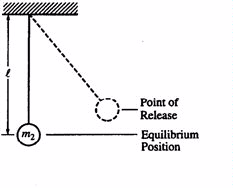
\includegraphics[keepaspectratio]{2004-APB-Q06-left}
        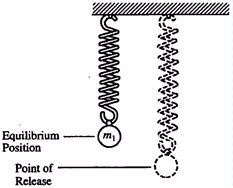
\includegraphics[keepaspectratio]{2004-APB-Q06-right}
    \end{center}
    Which of the following is true for both spheres?
    \begin{choices}
      \correctchoice{The maximum kinetic energy is attained as the sphere
                        passes through its equilibrium position.}
        \wrongchoice{The maximum kinetic energy is attained as the sphere
                        reaches its point of release.}
        \wrongchoice{The minimum gravitational potential energy is attained
                        as the sphere passes through its equilibrium position.}
        \wrongchoice{The maximum gravitational potential energy is attained
                        when the sphere reaches its point of release.}
        \wrongchoice{The maximum total energy is attained only as the sphere
                        passes through its equilibrium position.}
    \end{choices}
\end{question}
} 
